% 2017_national_paper_1_liberal_q18_fig1: pyramid P-ABCD, schematic oblique
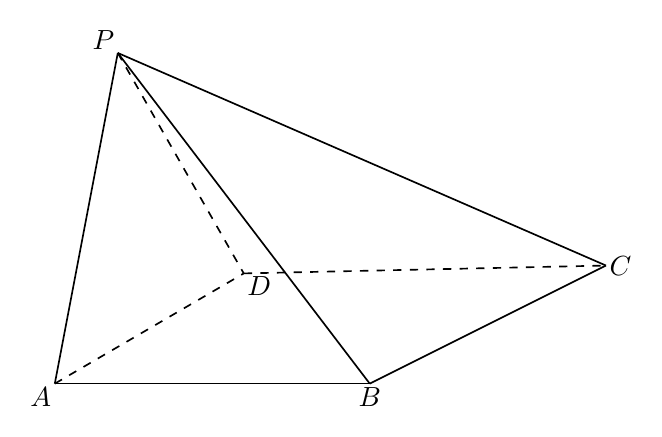
\begin{tikzpicture}[line width=0.6pt, font=\normalsize]
\coordinate (A) at (0,0);
\coordinate (B) at (4,0);
\coordinate (C) at (7,1.5);
\coordinate (D) at (2.4,1.4);
\coordinate (P) at (0.8,4.2);
% base front solid
\draw (A) -- (B);
\draw (B) -- (C);
% base hidden
\draw[dashed] (D) -- (C);
\draw[dashed] (A) -- (D);
% lateral solid
\draw (P) -- (A);
\draw (P) -- (B);
\draw (P) -- (C);
% lateral hidden
\draw[dashed] (P) -- (D);
% labels
\node[below left, inner sep=1pt] at (A) {$A$};
\node[below, inner sep=1pt] at (B) {$B$};
\node[right, inner sep=1pt] at (C) {$C$};
\node[below right, inner sep=1pt] at (D) {$D$};
\node[above left, inner sep=1pt] at (P) {$P$};
\end{tikzpicture}
